\documentclass[12pt]{article}
\usepackage[utf8]{inputenc}
\usepackage[T1]{fontenc}
\usepackage{amsmath, amssymb, geometry, tikz, booktabs, array}
\geometry{margin=1in}
\setlength{\parindent}{0pt}
\renewcommand{\arraystretch}{1.3}

% TikZ libraries needed for 'below=of' syntax and neat arrows/boxes
\usetikzlibrary{positioning}

\begin{document}

% ======================================================
% PAGE 1 — CONCEPTUAL SUMMARY
% ======================================================

\begin{center}
\Large \textbf{Summary of Major Trade Models} \\[4pt]
\normalsize (Ricardian, Specific-Factors, Heckscher--Ohlin, and Standard Trade Models)
\end{center}

\vspace{0.8em}

\section*{Overview}

International trade theory evolves through four core models. Each adds complexity by modifying assumptions about \textbf{factors of production}, \textbf{mobility}, and \textbf{sources of trade}.

\vspace{1em}

\begin{tabular}{>{\bfseries}p{3cm} p{3.5cm} p{2.6cm} p{2.4cm} p{3.1cm}}
\toprule
Model & Source of Trade & Factors of Production & Factor Mobility & Key Insights \\
\midrule
Ricardian & Technological differences & Labour only & Labour mobile across sectors & Comparative advantage; all workers gain. \\[3pt]

Specific-Factors & Short-run immobility of capital/land & Labour, capital, land (sector-specific) & Labour mobile; others fixed & Trade benefits export-sector owners, hurts import-sector owners. \\[3pt]

Heckscher--Ohlin & Relative factor endowments & Labour and capital & Both mobile & Countries export goods using abundant factors; factor price equalization. \\[3pt]

Standard Trade Model & Combination of technology, endowments, and preferences & Generalized factors & Flexible mobility assumption & Links production, demand, and terms of trade; unifies previous models. \\
\bottomrule
\end{tabular}

\vspace{1em}
\newpage
\section*{Income Distribution Effects}
\begin{itemize}
\item \textbf{Ricardian:} No inequality; all workers gain.
\item \textbf{Specific-Factors:} Export-sector owners gain, import-sector owners lose.
\item \textbf{Heckscher--Ohlin:} Abundant factor gains, scarce factor loses (Stolper--Samuelson).
\item \textbf{Standard Trade Model:} Distributional effects depend on bias of growth and movement in terms of trade.
\end{itemize}

\vspace{1em}

\section*{Conceptual Evolution Diagram}

\begin{center}
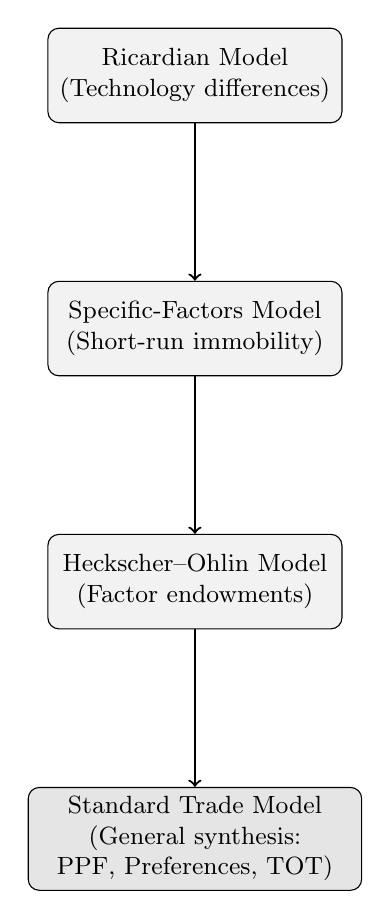
\begin{tikzpicture}[
  node distance=2cm,
  every node/.style={align=center, font=\small, rounded corners, draw, fill=gray!10, text width=3.5cm, minimum height=1.2cm}
]
\node (R) {Ricardian Model \\ (Technology differences)};
\node (S) [below=of R] {Specific-Factors Model \\ (Short-run immobility)};
\node (H) [below=of S] {Heckscher--Ohlin Model \\ (Factor endowments)};
\node (ST) [below=of H, fill=gray!20, text width=4cm] {Standard Trade Model \\ (General synthesis: PPF, Preferences, TOT)};

\draw[->, thick] (R) -- (S);
\draw[->, thick] (S) -- (H);
\draw[->, thick] (H) -- (ST);
\end{tikzpicture}
\end{center}

\vspace{0.6em}

\textit{The Standard Trade Model synthesizes all prior frameworks by linking production (PPF), demand (indifference curves), and world prices (terms of trade).}

\newpage

% ======================================================
% PAGE 2 — MATHEMATICAL FOUNDATIONS
% ======================================================

\begin{center}
\Large \textbf{Mathematical Foundations of the Major Trade Models}
\end{center}

\vspace{0.8em}

\section*{1. Ricardian Model}

\textbf{Assumptions:}
\begin{itemize}
\item Labour is the only factor; technology differs across countries.
\item Constant unit labour requirements \( a_{LX}, a_{LY} \).
\item Perfect competition \(\Rightarrow\) goods prices reflect labour costs.
\end{itemize}

\textbf{Equations:}
\[
\begin{aligned}
L_X + L_Y &= \bar{L}, \\
a_{LX} X + a_{LY} Y &= \bar{L}, \\
\frac{P_X}{P_Y} &= \frac{a_{LX}}{a_{LY}} \quad \text{(in autarky)}.
\end{aligned}
\]
Trade occurs when relative prices differ:
\[
\frac{a_{LX}}{a_{LY}} \neq \frac{a_{LX}^*}{a_{LY}^*}.
\]

\textbf{Result:} Specialization by comparative advantage; world production and welfare rise.

\vspace{1em}

\section*{2. Specific-Factors Model}

\textbf{Assumptions:}
\begin{itemize}
\item Two goods: \( M \) (manufactures) and \( A \) (agriculture).
\item Labour \( L \) is mobile; capital \( K \) specific to \( M \), land \( T \) specific to \( A \).
\end{itemize}

\textbf{Production functions:}
\[
Q_M = Q_M(K, L_M), \quad Q_A = Q_A(T, L_A), \quad L_M + L_A = \bar{L}.
\]

\textbf{Wage equalization:}
\[
P_M \, MPL_M = P_A \, MPL_A = w.
\]
\textbf{Implications:}
\begin{itemize}
\item An increase in \( P_M/P_A \) shifts labour toward \( M \).
\item \( r_K \) (return to capital) rises; \( r_T \) (return to land) falls.
\item Labour's real wage effect is ambiguous.
\end{itemize}

\vspace{1em}

\section*{3. Heckscher--Ohlin Model}

\textbf{Assumptions:}
\begin{itemize}
\item Two factors: \( L \) and \( K \); both mobile.
\item Two goods: \( X \) (labour-intensive) and \( Y \) (capital-intensive).
\item Identical technologies across countries; different factor endowments.
\end{itemize}

\textbf{Zero-profit conditions:}
\[
\begin{aligned}
P_X &= a_{LX} \, w + a_{KX} \, r, \\
P_Y &= a_{LY} \, w + a_{KY} \, r.
\end{aligned}
\]
Given \( P_X/P_Y \), solve for \( w/r \).

\textbf{Key Theorems:}
\begin{itemize}
\item \textbf{Heckscher--Ohlin:} Countries export goods using their abundant factor intensively.
\item \textbf{Stolper--Samuelson:} A rise in the price of a good raises the real return to the factor used intensively in that good.
\item \textbf{Rybczynski:} An increase in one factor endowment increases output of the good using that factor intensively.
\end{itemize}

\vspace{1em}

\section*{4. Standard Trade Model}

\textbf{Purpose:} Combine production, demand, and world prices in one unified framework.

\textbf{Relative supply (RS) and relative demand (RD):}
\[
RS = \frac{Q_X}{Q_Y} = f\!\left(\frac{P_X}{P_Y}\right), \qquad RD = \frac{D_X}{D_Y} = g\!\left(\frac{P_X}{P_Y}\right).
\]

\textbf{Equilibrium:}
\[
RS = RD \quad \Rightarrow \quad \frac{P_X}{P_Y} = \left(\frac{P_X}{P_Y}\right)^{W}.
\]

\textbf{Terms of Trade (TOT):}
\[
\text{TOT} = \frac{P_{\text{exports}}}{P_{\text{imports}}}.
\]

\textbf{Welfare:}
Improvement in TOT \(\Rightarrow\) outward pivot of trade line \(\Rightarrow\) higher indifference curve.  
Growth or policy shifts RS/RD, altering equilibrium prices and welfare.

\textbf{Graphically:} Welfare at tangency of highest indifference curve with world price line tangent to PPF.



\end{document}
